\section{Presentation-Abstraction-Control}


Das Presentation-Abstraction-Control Pattern (PAC) definiert eine Struktur für interaktive Anwendungen in Form einer Hierarchie von kooperierenden Agents (Agenten). Jeder Agent ist Verantwortlich für ein Aspekt der Anwendungsfunktionalität und besteht aus drei Komponenten: Presentation, Abstraction und Control. Diese Unterteilung trennt die Benuterzschnittstellen-Interaktionsaspekte des Agents von seinem funktionalen Kern und seiner Kommunikation mit anderen Agents.

\subsection*{Example}


Bei einem Informationssystem für politischen Wahlen wollen wir Daten proportional anzeigen. Dazu haben wir eine Tabelle um Daten einzugeben und mehrere Diagramme um die aktuellen Ergebnisse zu präsentieren. Benutzer interagieren mit der Software über eine grafische Schnittstelle.

Verschiedene Versionen passen jedoch die Benutzerschnittstelle spezifisch an. Zum Beispiel kann eine Version zusätzliche Views der Daten anzeigen, wie die Zugehörigkeit von Parlamentssitzen zu Parteien.

\subsection*{Context}


Entwickle eine interaktive Anwendung mit der Hilfe von Agents (Agenten).

\subsection*{Problem}


Interaktive Systeme können oft als eine Menge von kooperierenden Agents angesehen werden. Agents sind spezialisiert in der Mensch-Maschinen-Interaktion, akzeptieren Benutzereingaben und zeigen Daten an. Weitere Agents sind verantwortlich für verschiedene Aufgaen, wie Fehlerbehandlung (Error Handling) oder Kommunikation mit anderen Software-Systemen. Neben dieser horizontalen Aufteilung treffen wir oft auch eine vertikale Aufteilung des Systems an.

In einer Architektur mit kooperierenden Agents ist jeder Agent auf eine bestimmte Aufgabe spezialisiert. Alle Agents zusammen stellen die Funktionalität des Systems zur verfügung. Dieses Architektur umfasst sowohl eine horizontale, wie auch eine vertikale Aufteilung.

\subsection*{Forces}


\begin{itemize}
	\item Agents verwalten oft ihren eigenen Zustand sowie ihre Daten.
	\item Interaktive Agents stellen ihre eigene Benutzerschnittstelle zur Verfügung.
	\item Systeme entwickeln sich über die Zeit. Vor allem die Präsentation ist anfällig für Änderungen.
\end{itemize}

\subsection*{Solution}


Strukturiere die interaktive Anwendung als baumartige Hierarchie von PAC Agents. Dabei sollen ein Top-Level-Agent, mehrere Intermediate-Level-Agents und noch mehr Bottom-Level-Agents existieren. Jeder Agent ist verantwortlich für einen bestimmten Aspekt der Anwendungsfunktionalität und besteht aus drei Komponenten: Presentation, Abstraction und Control.

Die ganze Hierarchie widerspiegelt transitive Abhängigkeiten zwischen Agents. Jeder Agent ist von allen Higher-Level-Agents abhängig.

Die Presentation-Komponente eines Agents stellt dessen sichtbares Verhalten dar. Seine Abstraction-Komponente verwaltet dessen Datenmodel und stellt darauf zugreifende Funktionalität zur Verfügung. Die Control-Komponent

Die Top-Level-Komponente stellt die Grundfunktionalität des Systems zur Verfügung. Die meisten anderen PAC Agents hängen von ihr ab oder arbeiten mit ihr. Zudem enthält der Top-Level PAC Agent die teile der Benutzerschnittstelle, welche nicht einer bestimmten Unteraufgabe zugeordnet werden können.

Bottom-Level PAC Agents repräsentieren in sich abgeschlossene, semantische Konzepte mit denen der Benutzer arbeiten kann, wie Tabellen order Diagramme.

Intermediate-Level PAC Agents stellen entwender Kominationen oder Beziehungen von niedrigeren Agents dar. So kann zum Beispiel ein Intermediate-Level-Agent verschiedene Views auf die selben Daten verwalten.

\begin{figure}[H]
	\centering
	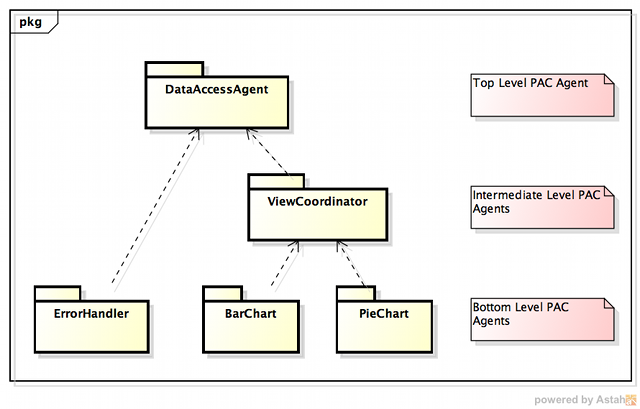
\includegraphics[width=0.7\textwidth]{content/posa1/images/presentation-abstraction-control-overview.png}
	\caption{Overview}
\end{figure}


\subsection*{Structure}


Die Hauptverantwortung des Top-Level PAC Agent ist das globale Modell der Software zur Verfügung zu stellen. Dises wird in der Abstraction-Komponente des Top-Level-Agent verwaltet. Die Schnittstelle der Abstraction-Komponente bietet Funktonen an um das Datenmodel zu manipulieren.

Die Presentation-Komponente des Top-Level Agent beinhaltet allgemeine Benutzerschnittstellen Elemente der ganzen Anwendung. In einigen Systemen existiert keine Top-Level Presentation-Komponente.

Die Control-Komponente des Top-Level PAC Agent hat drei Aufgaben:

\begin{itemize}
	\item Sie erlaubt niedrigere Agents die Verwendung von Diensten der Top-Level Agents, wie zum Beispiel das manipulieren des globalen Daten-Modells. Anfragen werden entwder zur Abstraction- oder zur Presentation-Komponente weitergeleitet.
	\item Sie koordiniert die Hierarchie der PAC Agents.
	\item Sie verwaltet informationen über die Interaktion des Benutzers mit dem System.
\end{itemize}

Bottom-Level PAC Agents repräsentiere bestimmte, semantische Konzepte der Anwendungsdomäne.

Die Presentation-Komponente eines Bottom-Level-PAC Agents präsentiert die View auf das entsprechende semantische Konzept und stellt den Zugriff des Benutzers auf diese zur Verfügung. Intern kann die Presentation-Komponete auch Informationen über die View selbst beinhalten, wie z.B eine Bildschirmposition.

Die Abstraction-Komponente eines Bottom-Level-PAC Agents hat eine ähnliche Aufgabe wie die Abstraction-Komponente des Top-Level-PAC Agent. Im Unterschied zu dieser sind allerdings keine anderen PAC-Agents von diesen Daten abhängig.

Die Control-Komponente des Bottom-Level PAC Agent verwaltet die Konsistenz zwischen der Abstraction- und der Presentation-Komponente wodurch sie direkte Abhängikeiten dieser zueinander vermeidet. Sie kommuniziert mit höheren Agents um Ereignisse (Events) und Daten auszutauschen. Eingehende Ereignisse, wie die Anforderung ein Fenster zu schliessen werden weiergeleitet zur Presentation-Komponente des Bottom-Level Agent. Ausgehende Ereignisse und Daten wie zum Beispiel Fehlermeldungen werden zum entsprechenden, höheren Agent gesendet.

\begin{figure}[H]
	\centering
	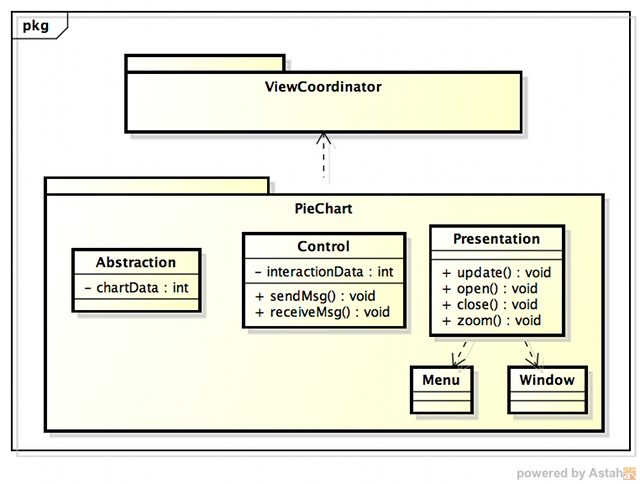
\includegraphics[width=0.7\textwidth]{content/posa1/images/presentation-abstraction-control-details.png}
	\caption{Detail}
\end{figure}


\subsection*{Dynamics}


Szenario 1: Kooperation zwischen verschiedenen PAC Agents eim öffnen einer Balkendiagramm-View von Wahl-Daten.

:: UML Diagramm von Seite 154? ::

\begin{enumerate}
	\item Der Benutzer verlangt von der Presentation-Komponente des View-Koordinations-Agent ein neues Balkendiagramm zu öffnen.
	\item Die Control-Komponente des View-Koordinations-Agent erstellt eine neue Instanz des gewünschten Balkendiagramm-Agent.
	\item Der View-Koordinations-Agent sendet ein "Öffnen"/"Open" Ereignis zur Control-Komponente des neue Balkendiagramm-Agent.
	\item Die Control-Komponente des Balkendiagramm-Agent bekommt als erstes Daten vom Top-Level PAC Agent. Der View-Koordinations-Agent vermittelt zwischen Bottom- und Top-Level-Agents. Die Daten speichert der Balkendiagramm-Agent in seiner Abstraction-Komponente. Seine Control-Komponente ruft daraufhin die Presentation-Komponente auf um das Diagramm anzuzeigen.
	\item Die Presenation-Komponente erstellt eine neues Fenster auf dem Bildschirm, erhält die Daten von der Abstraction-Komponente in dem es sie von der Control-Komponente anfordert, um sie schliesslich im neuen Fenster anzuzeigen.
\end{enumerate}


:: UML Diagramm von Seite 155? ::

\begin{enumerate}
	\item Der Benutzer gibt neue Daten in eine Tabelle ein. Die Control-Komponente der Tabellen-Agent leitet diese Daten an den Top-Level PAC Agent weiter.
	\item Die Control-Komponente des Top-Level PAC Agent erhält die Information und weist die Abstaction-Komponente an die gespeicherten Daten entsprechend zu ändern. Die Abstaction-Komponente des Top-Level Agent weist daraufhin die Control-Komponte an, alle Agenten zu informieren, welche von diesen neuen Daten abhängig sind.
	\item Die Control-Komponente des View-Koordinator Agent leitet die Benachrichtigung an alle View-PAC Agents weiter.
	\item Die View-PAC Agents aktualisieren ihre Daten und zeigen diese auf dem Bildschirm an.
\end{enumerate}


\begin{enumerate}
	\item  Definiere ein Model der Anwendung.
	\item  Definiere eine allgemeine Strategie um die PAC Hierarchie zu organisieren.
	\item  Spezifiziere den Top-Level PAC Agent.
	\item  Spezifiziere die Bottom-Level PAC Agents.
	\item  Spezifiziere Bottom-Level PAC Agents für System Dienste, welche nicht direkt dem Ziel des Systems dienen.
	\item  Spezifiere Intermediate-Level PAC Agents welche die Bottom-Level PAC Agents zusammenhalten. Oft bilden mehrere Bottom-Level PAC Agents zusammen ein semantisches Konzept.
	\item  Spezifiziere Intermediate-Level PAC Agents welche Lower-Level PAC Agents koordinieren.
	\item  Trenne die Grundfunktionalität von der Mensch-Maschinen-Interaktion.
	\item  Stelle eine externe Schnittstelle zur Verfügung.
	\item Verbinde die Hierarchie. Nach dem die individuellen PAC Agents implementiert wurden kann man die letztendliche PAC-Hierarchie aufbauen.
\end{enumerate}


\begin{itemize}
	\item PAC agents as active objects. Jeder PAC Agent als eigener Thread. Das Active Object Pattern und das Half-Sync/Half-Async Pattern können dabei hilfreich sein.
	\item PAC agents as processes. Jeder PAC Agent als eigener Prozess, möglicherweise auch remote auf anderen Rechnern. Das Proxy Pattern hilft dabei direkte Abhängigkeiten zu vermeiden. Mit dem Forwarder-Receiver Pattern order dem Client-Dispatcher-Server Pattern lässt sich die Interprozess Kommunikation (ICP) zwischen den PAC agents lösen. Falls IPC zu ineffizient ist, können ganze, zusammenhängende Teilbäume der PAC-Hierarchie in eigene Prozesse ausgelagert werden. IPC zwischen PAC Agents wird dadurch minimiert.
\end{itemize}

\subsection*{Known Uses}


\begin{itemize}
	\item Netzwerk Traffic Management
	\item Mobile Robot
\end{itemize}

\subsection*{Consequences}


\subsubsection*{Benefits}


\begin{itemize}
	\item Separation of concerns. Verschiedene semantische Konzepte der Anwendungsdomäne werden durch eigene Agents repräsentiert.
	\item Support for change and extension. Änderungen in den Presentation- oder Abstraction-Komponenten haben keine Auswirkungen auf andere Agents im System.
	\item Support for multi-tasking. PAC agents können einfach auf verschiedene Thread, Prozesse oder Rechner verteilt werden. Die Änderungen betreffend der entsprechenden IPC-Funktionalität eines Agents betreffen seine Control-Komponente.
\end{itemize}

\subsubsection*{Liablities}


\begin{itemize}
	\item Increased system complexity. Die Implementation jedes semantischen Konzepts einer Anwendung durch eigene PAC Agents kann in einer sehr komplexen System-Struktur resultieren.
	\item Complex control component. Die Qualität der Control-Komponenten ist entscheident für eine effektive Zusammenarbeit zwischen Agents und dementsprechend auch für die des gesamten Systems.
	\item Efficiency. Der Overhead bei der Kommunikation zwischen PAC Agents kann sich negativ auf die Effizienz des Systems auswirken.
	\item Applicability. Je kleiner die eigenständigen, semantischen Konzepte einer Anwendung sind, desto grösser ist die Ähnlichkeit ihrer Benutzerschnittstelle, desto weniger lässt sich dieses Pattern anwenden.
\end{itemize}

\subsection*{See also}


Auch das Model-View-Controller Pattern (MVC) trennt die Grundfunktionalität eines Software Sytems von der Anzeige der Informationen und der Verarbeitung von Benutzereingaben. MVC definiert seinen Controller allerdings als Entität welche für das Entgegennehmen von Benutzereingaben verantwortlich ist. Dies bedeutet, dass MVC den vom Benutzer verwendeten Teil des Systems - die Presentation-Komponente beim PAC Pattern - in eine View- und einen Control-Komponente teilt. Desweiteren unterteilt MVC eigenständige Unteraufgaben eines Systems nicht in kooperiende, aber lose gekoppelte Agents.

\subsection*{Mögliche Prüfungsfragen}


(ev. wodurch hebt es sich von mvc ab?)
